\chapter{Methods:}

\section{Model overview:}

In order to investigate the seasonal variations of \ch{CO2} and ocean \ch{pCO2} fluxes with enhanced alkalinity, output data from two model simulations were provided by GEOMAR Helmholtz Zentrum für Ozeanforschung (Kiel, Germany) in a netCDF format and analysed using Python programming language. This manuscript is therefore accompanied by a Data Management Plan that follows the outline provided by Wageningen University. Additionally, all scripts will be made freely available on the author's GitHub repository to allow for replication and encourage open-source research. 

The data used for this manuscript is derived from the \ac{foci} model, an emission-driven \ac{esm} that consists of an atmosphere, an ocean and a land surface component. The atmosphere is divided into 95 vertical layers and the ocean into 46 vertical layers, and the two components are coupled by the model every three hours. The ocean model has a spatial resolution of 1/2\textdegree{} on a tripolar grid. 

\ac{foci} incorporates the \ac{mops} to enable the simulation of marine biogeochemical cycles (\cref{foci-mops}) \citep{chien2022foci}. In its primitive version, \ac{mops} simulated the elemental cycle of phosphorous, nitrogen, and oxygen. When integrated into \ac{foci}, a full carbon cycle including \ac{dic} and alkalinity tracers was implemented. This allowed to resolve biological dynamics such as phytoplankton uptake and remineralisation, calcite formation and dissolution. \ac{foci}-\ac{mops} undergoes a 500-year spin-up, after which steady state is achieved for all variables, with the commonly-observed exception of nitrogen \citep{chien2022foci}.

\begin{figure}[H]
\caption[Schematic of the biogeochemistry in \texorpdfstring{FOCI}{FOCI}-\texorpdfstring{MOPS}{MOPS}.]{Schematic of the biogeochemistry in \ac{foci}-\ac{mops}. Arrows represent the interactions between different compartments.}
\label{foci-mops}
\centering
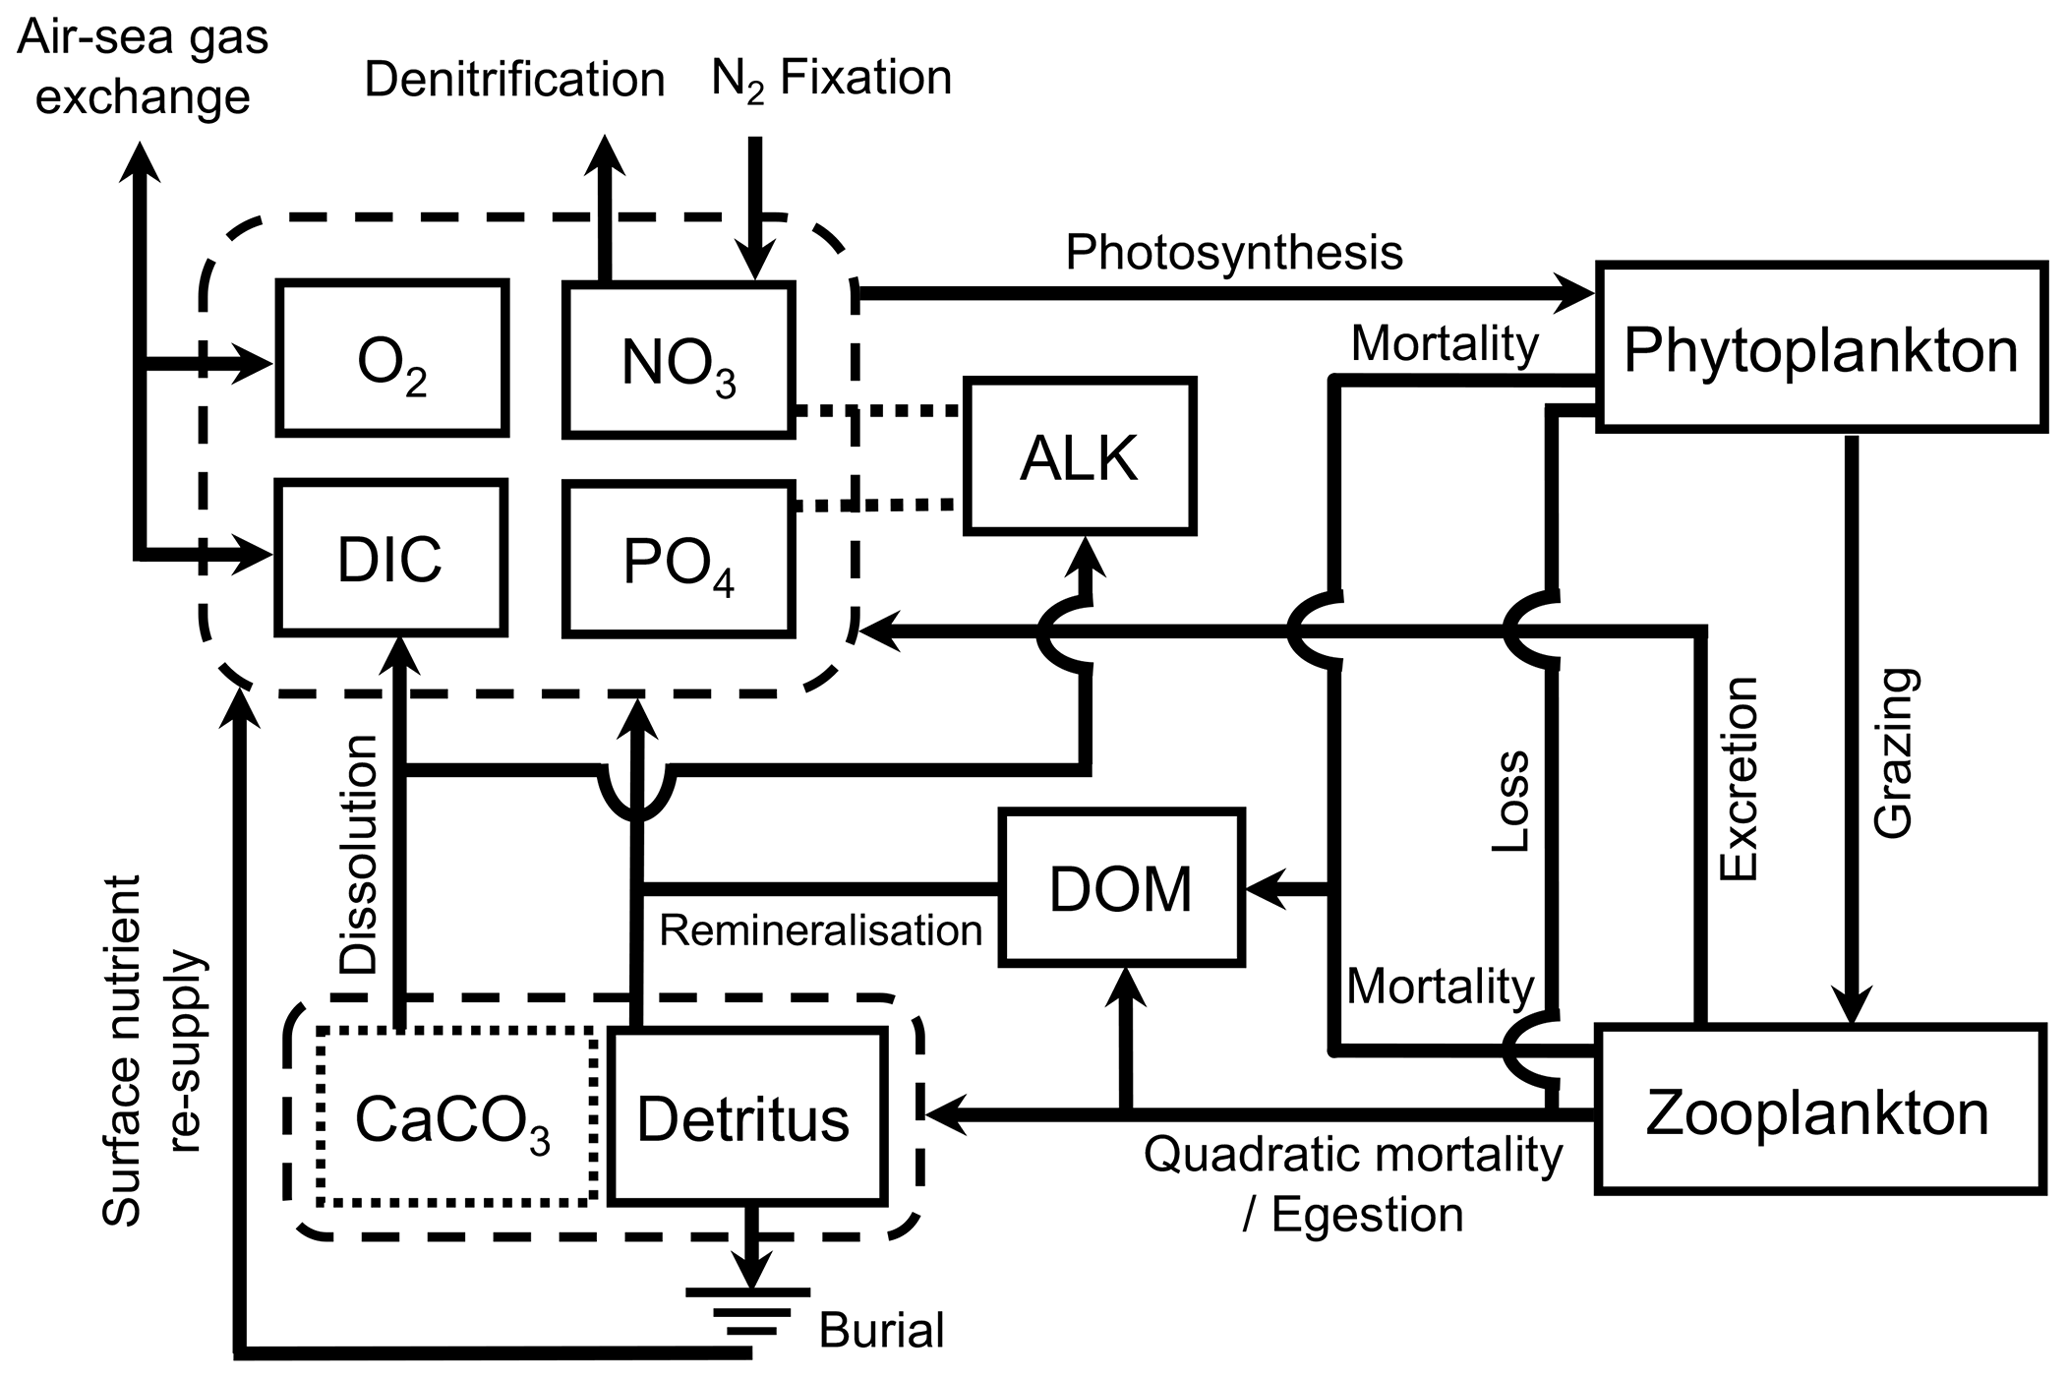
\includegraphics[width=12cm]{fig/1_Introduction/foci-mops.png}

\scriptsize Source: \cite{chien2022foci}
\end{figure}

Historical simulations were run from the year 1850 to the year 2015, from which the \ac{ssp} scenarios start. The simulations with alkalinity addition begin in year 2025 until 2100, with monthly time-steps. Alkalinity addition is simulated along the European coastline of 50-kilometre width, with the exclusion of the Baltic and the Mediterranean seas that are poorly resolved by the model. In \ac{foci}, alkalinity is a prognostic tracer simulated as a combination of biological sources and sinks: nitrate and phosphate supply as sinks, calcium carbonate production and dissolution as sink and source, respectively, and \ac{om} formation and remineralisation, as sink and source, respectively (\cref{foci-mops}) \citep{chen2021quantifying}. 

Two baseline \ac{ssp} scenarios were considered for the analysis. The first is SSP1-2.6 and describes a low-emission future with a radiative forcing of 2.6 W m\textsuperscript{-2} by the end of the century. This scenario prescribes strong emission abatement policies and reaches a limited warming below 2\textdegree C. The second is SSP3-7.0 and narrates a high-emission future with a radiative forcing of 7.0 W m\textsuperscript{-2} by 2100. This scenario lacks ambitious emission reduction strategies, implies relatively strong land use change and has a warming potential of about 4\textdegree C compared to pre-industrial levels \citep{o2016scenario}. 

\ac{oae} is simulated in \ac{foci} using a masking approach. Alkalinity is added to the system continuously and uniformly along the European coast (blue bordering line in \cref{oaemodel}) through the incorporation of fast-reacting quicklime on the ocean surface which is then allowed to diffuse over the domain. Alkalinity addition is subject to a linear increase over a 10-year period until the equivalent of 1 Gt yr\textsuperscript{-1} of calcium hydroxide (\ch{Ca(OH)2}) is reached. The latter consumes two moles of atmospheric \ch{CO2} and produces one mole of calcium (\ch{Ca}\textsuperscript{2+}) and two moles of bicarbonate ions (\ch{HCO3-}), therefore ideally increasing alkalinity by a factor of two (see \eqref{eqn:calc}) \citep{chien2022foci}. 

\begin{center}

\begin{equation} 
\label{eqn:calc}
\ch{Ca(OH)2} + 2\ch{CO2} \leftrightarrow \ch{Ca}\textsuperscript{2+} + 2\ch{HCO3-}
\end{equation}

\end{center}

\begin{figure}[H]
\caption[\texorpdfstring{OAE}{OAE} application in the study area]{Geographical \ac{oae} application in the study area}
\label{oaemodel}
\centering
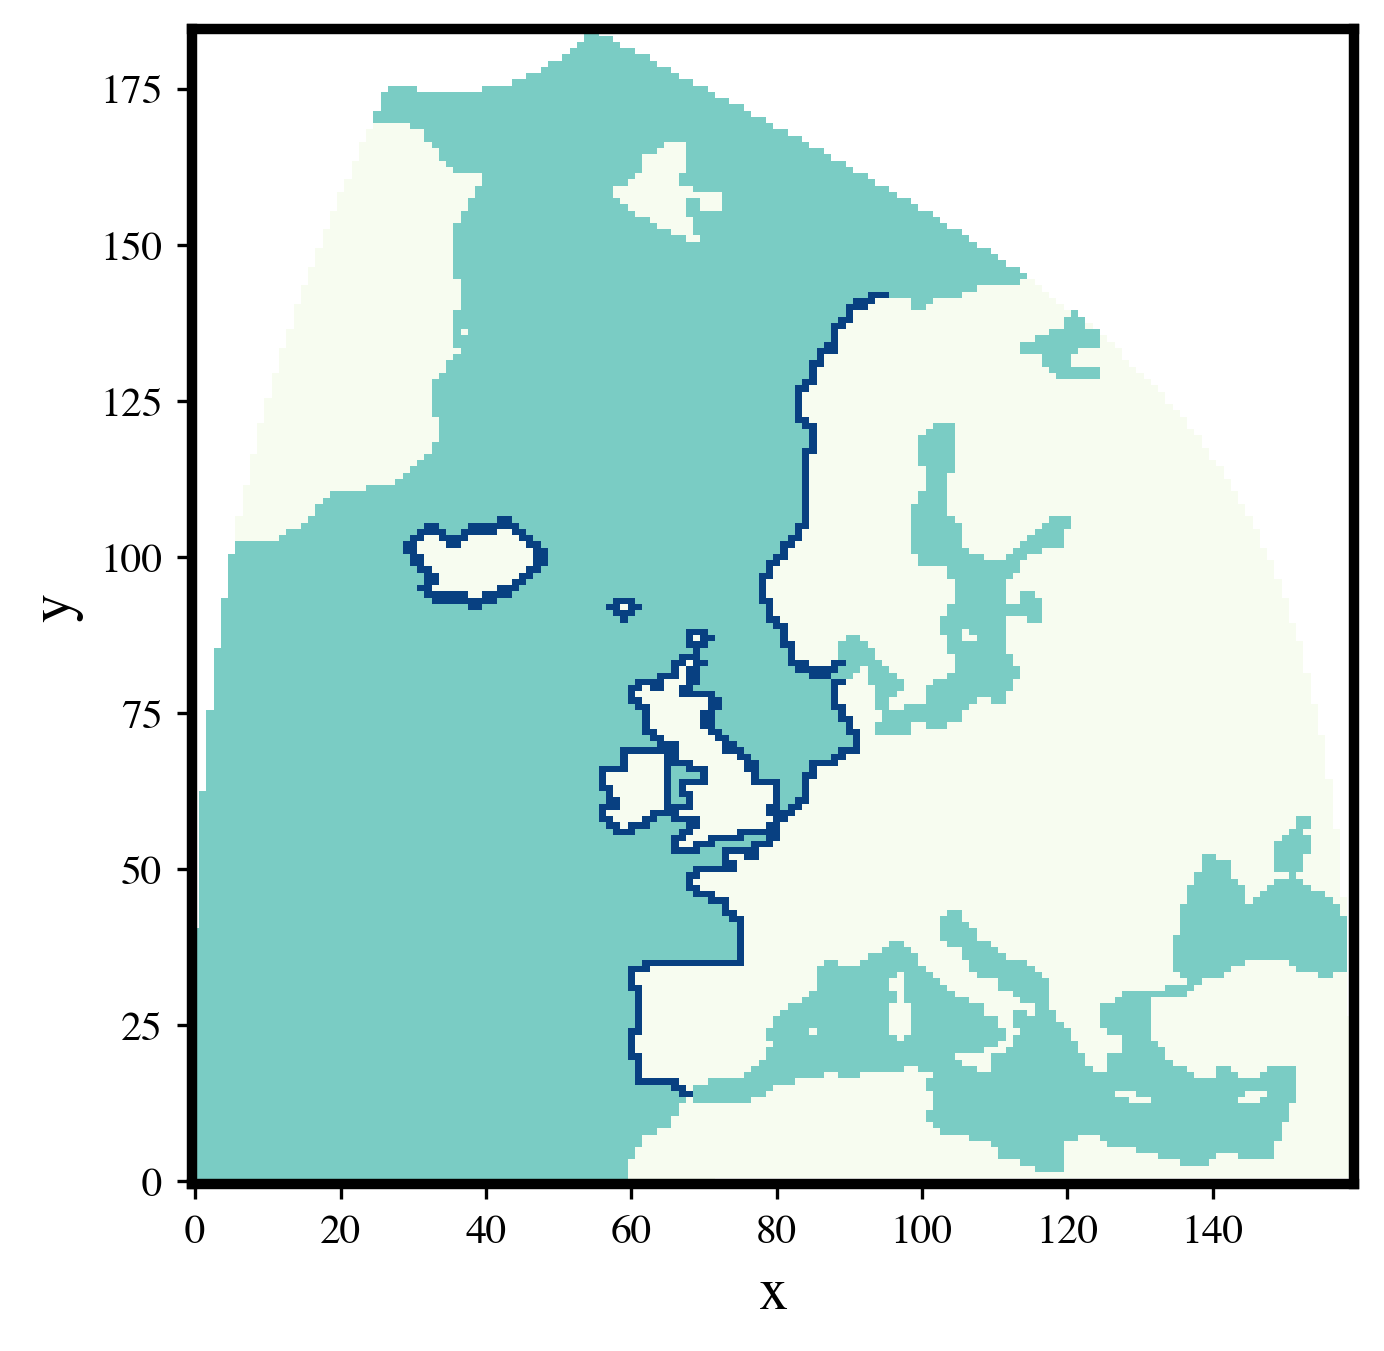
\includegraphics[width=10cm]{fig/2_Methods/mesh_mask_area.png}

\end{figure}

The parameterisation of air-sea gas exchange in \ac{foci} is described by the following equation:

\begin{center}

\begin{equation}
\label{eqn:1.1}
F_{ \ch{CO2} }  =  k_{w} ([ \ch{CO2*}]_{sat} -[ \ch{CO2*}]) 
\end{equation}

\end{center}

where $ k_{w} $ is the gas transfer velocity in m s\textsuperscript{-1}, $ \ch{CO2*}_{sat} $ is the saturation concentration of \ch{CO2} in mol kg\textsuperscript{-1}, and $ \ch{CO2*} $ is the surface ocean dissolved \ch{CO2} concentration in mol kg\textsuperscript{-1} \citep{chien2022foci}.

Ocean \ch{pCO2}, that in \ac{foci} is termed surface \ch{CO2} fugacity, is calculated as follows:

\begin{center}

\begin{equation}
\label{eqnfCO2}
f{ \ch{CO2} } = \ch{CO2*} / K\textsubscript{0} 
\end{equation}
    
\end{center}

where K\textsubscript{0} is the solubility coefficient of \ch{CO2} in seawater. Both factors are affected by a multitude of intertwined physical and biological processes which are sometimes difficult to analyse individually. Some of the variables may also be subject to over and underestimation, therefore altering connected interactions \citep{chien2022foci}. 

\section{Descriptive analysis and data pre-processing:}

The methodology of this study consists of a descriptive analysis and splits in two parts. First, the focus is put on the European area and seasonality is calculated to account for regional averages. Then, the analysis zooms in a specific geographical point termed S, which was arbitrarily assigned off of the Dutch coasts, at 52\degree N and 3\degree E (red circle in figure \Cref{cropping}). This is done with the aim of visualising the differences and similarities between the system as a whole and the epicentre of the experiment domain in the southern North Sea. 

The global output data was sliced to the European coastline, with coordinates -25\degree{} to 10\degree{} E and 40\degree{} to 70\degree{} N. As found in \cref{cropping}, the cropped area does not cover the entire European region where \ac{oae} was performed, and part of the Norwegian and Spanish littoral were left out of the analysis. This approximation was due to time constraints and does not result in a meaningful modification from the actual regional definition. 

\begin{figure}[H]
\caption[Cropping of the study area and geographical location of point S]{Cropping of the study area (left) and geographical location of point S (right)}
\label{cropping}
\centering
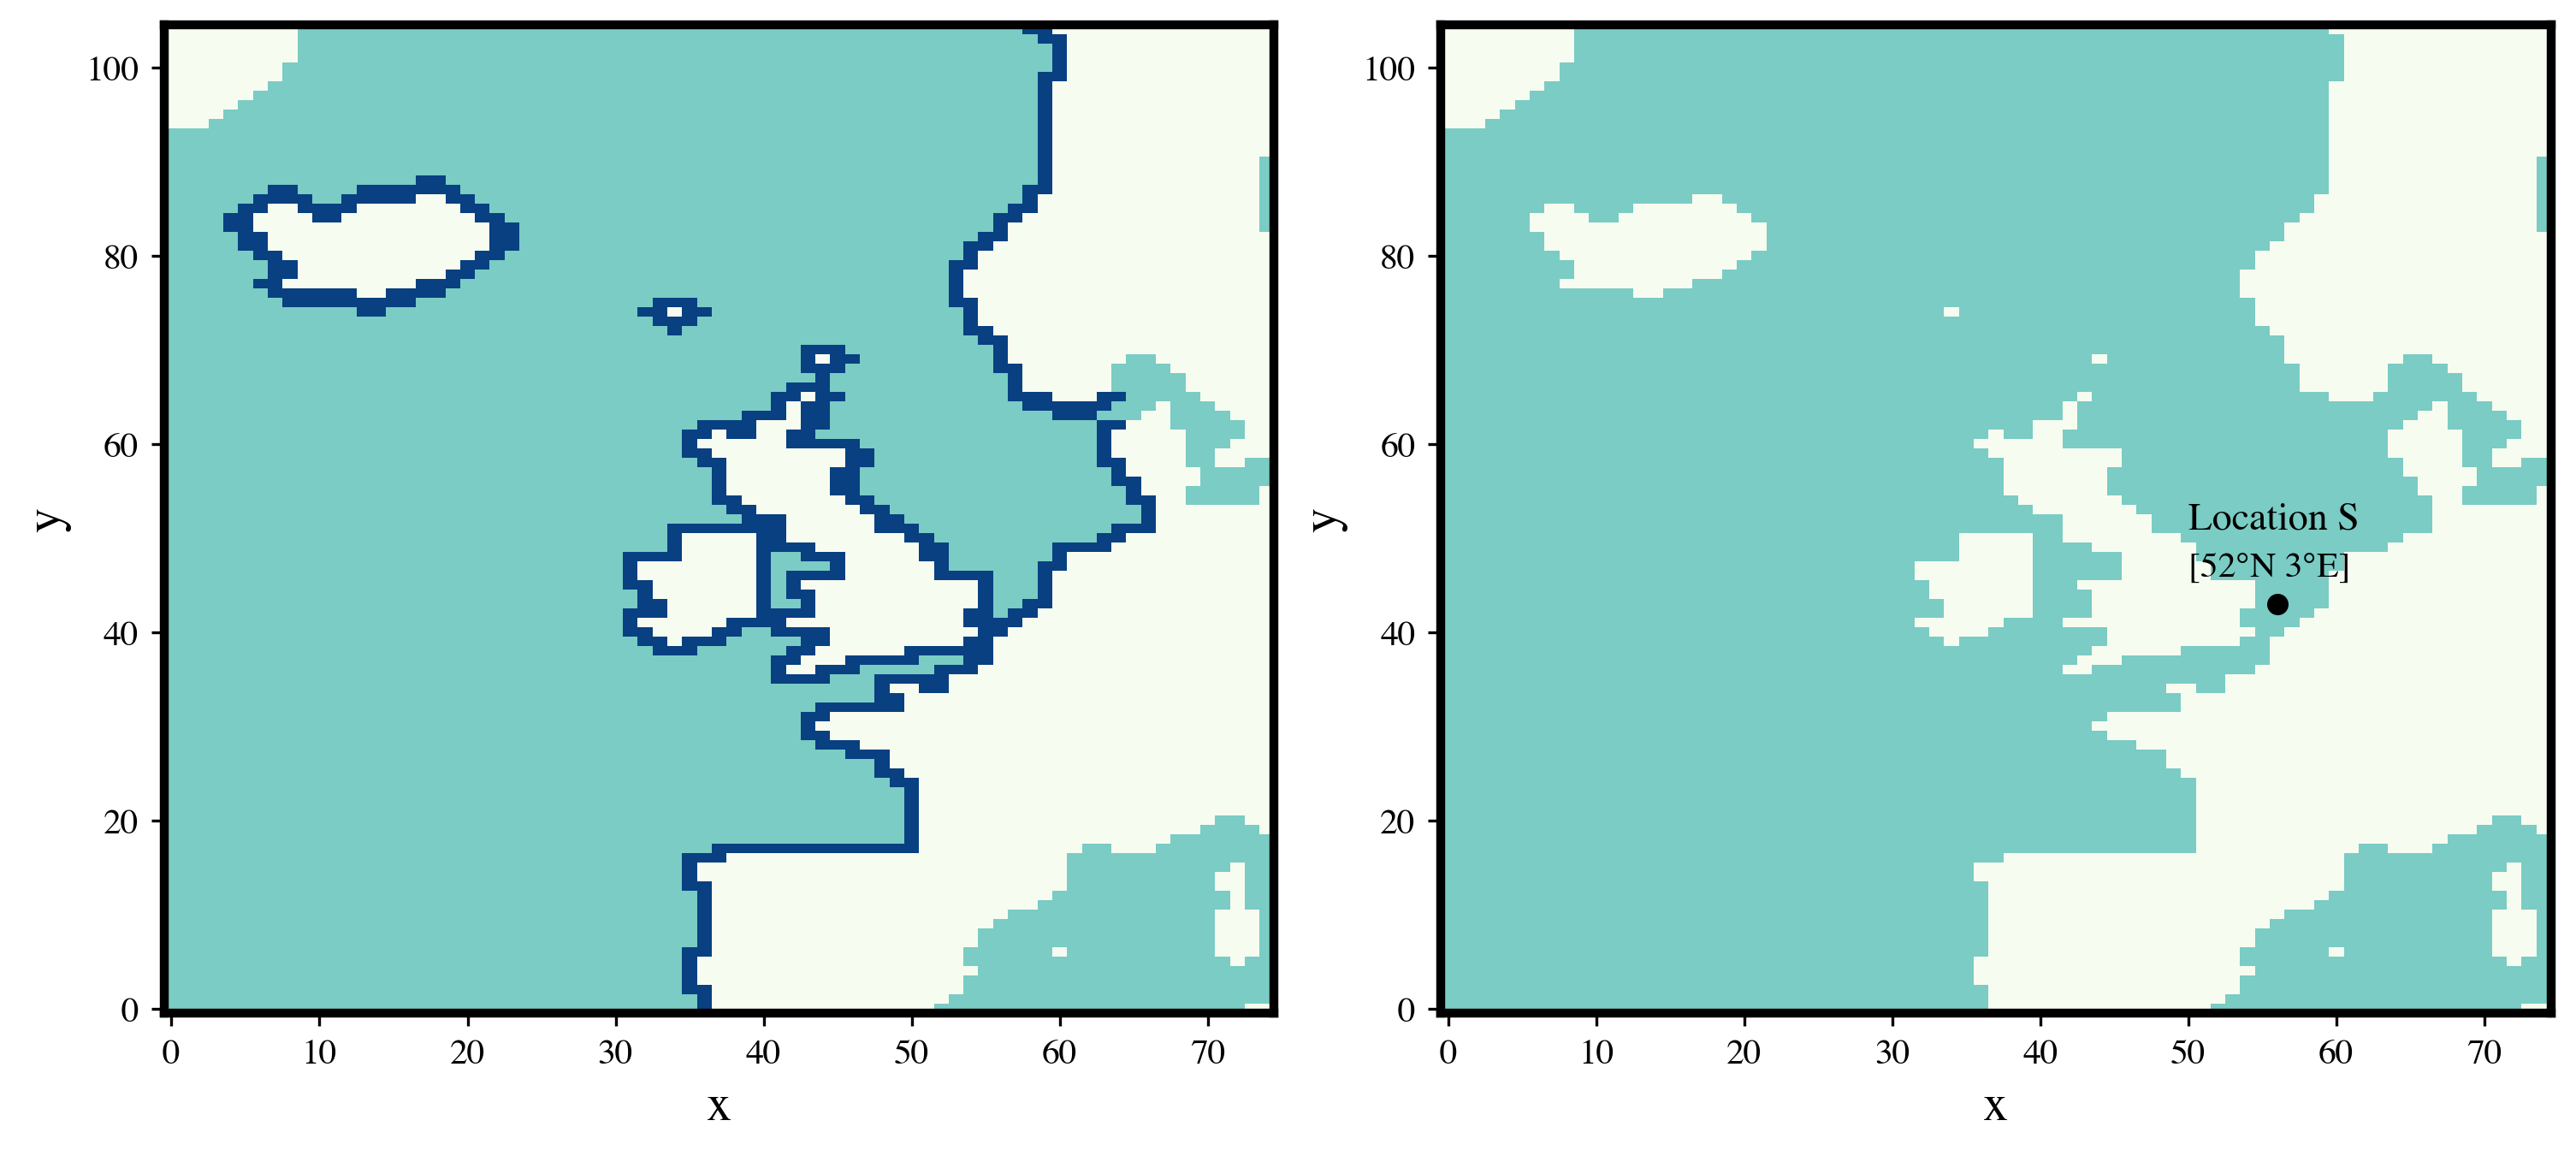
\includegraphics[width=15cm]{fig/2_Methods/mesh_mask_point.png}

\end{figure}

As previous studies suggest that seasonal trends detected at the ocean surface emerges after around ten years, a decadal trend investigation was conducted, drawing from \cite{wang2023simulated}. Additionally, seasonal discrepancies between the two scenarios were expected to be the most visible close to the simulation's end, when the system has stabilised. Therefore, the last 10 years registered by \ac{foci} (2090-2100) were selected. Due to a limited space, an annual average for the last decade is shown in this manuscript. 

Five main parameters were extracted from the simulation dataset, here presented in the order from drivers to outcome variables: alkalinity, pH, \ac{dic}, \ch{pCO2}, and \ch{CO2} flux. While \ch{CO2} flux, \ch{pCO2} and pH are designed 3-dimensionally, with a latitude, longitude and time dimension, \ac{dic} and alkalinity are also calculated over the 46 layers in which the ocean component of the model is divided. Therefore, the investigation of those variables takes the average over the ocean surface that was arbitrarily set at 50 metres. 

It is worth noting that, due to its shallow profile, in the southern North Sea, the depth of the water column is lower than 50 metres. At location S, for example, the maximum water depth goes as low as 16.3 m, which represents the third \ac{foci} layer. Additionally, in the model, each layer length increases as a function of depth, meaning a weighted average was performed over the selected range of 50 metres for alkalinity and \ac{dic}. 

A land mask was applied to discount all land values, which in the simulations correspond to 0 (with the exception of pH) and would therefore have altered the calculated absolute values. All variables were then re-averaged based on the grid cell area (for \ch{CO2} flux, \ch{pCO2} and pH) and volume (for \ac{dic} and alkalinity). Unlike the other four, \ch{CO2} flux calculations are performed in the atmospheric component of \ac{foci}, which has a grid resolution of $\sim$1.8\textdegree{}. This explains the coarser pattern in the \ch{CO2} flux plots presented below \citep{matthes2020flexible}.

To account for the volume of each grid cell, the units of \ac{dic} and alkalinity were transformed from µmol kg\textsuperscript{-1} to mmol m\textsuperscript{-3}. The datasets were divided by 1000 to convert µmol into mmol, and then multiplied by 1,025 kg m\textsuperscript{-3}, that is, global potential seawater density. As for \ch{CO2} flux, the \ac{foci} output delivers the variable in kg m\textsuperscript{-2} s\textsuperscript{-1}. Although such unit is dominating in climate mitigation literature, it is noted that, in ocean-focused papers, air-sea \ch{CO2} flux is usually measured in mol m\textsuperscript{-2} yr\textsuperscript{-1}. Therefore, the datasets were converted into such unit multiplying by the number of seconds in one year (31,536,000 seconds) and dividing by the molar mass of carbon dioxide in mol kg\textsuperscript{-1}, that is, 0.04401 mol kg\textsuperscript{-1}.

To account for seasonality, the monthly mean data were arranged in groups of three and averaged to the corresponding seasonal value. The four seasons were delineated as follows: winter, which includes December, January and February (DJF); spring, gathering March, April and May (MAM); summer includes June, July and August (JJA); finally, September, October and November compose autumn (SON). Seasonal trends were calculated with a weighting method, which accounted for the number of days contained in each month composing the target season. Then, the seasons were ungrouped to investigate monthly means and sub-seasonal variations, therefore gaining higher accuracy. Lastly, drawing from \cite{jo2022future}, seasonal amplitude regional maps were drawn, where the seasonal amplitude is the difference between the annual maximum and the annual minimum for the defined variable. 

Different descriptive tools were utilised to visualise the data. Scatterplots and lineplots define European and location S averages: in the former, local differences are approximated and give an overview of how the European system as a whole will behave in the future; in the latter, taking the average over location S allows to draw conclusions of regime shifts close to the epicentre of the domain. Additionally, maps were used to identify local patterns and distinguish the alkalised and non-alkalised ocean behaviour in different geographical areas accounting, for example, for the vicinity to the injection sites or the access to open-ocean regions.

\section{Overview of the explored variables:}

This section provides a short summary of the variables explored in this manuscript and their representation in the \ac{foci} model in the order from drivers to affected outcomes.

\begin{itemize}
    \item Alkalinity: it is the property that defines seawater capacity to neutralise pH changes. In \ac{foci}, alkalinity is measured in µmol kg\textsuperscript{-1}, which was converted in mmol m\textsuperscript{-3}. Alkalinity is analysed over depth, calculating the average of the surface water set at 50 metres for the European average, and at 16.3 metres for location S (corresponding to the third \ac{foci} depth layer).
    \item \ac{dic}: the \ac{dic} pool incorporates the three carbon species that the ocean stores, namely \ch{HCO3-}, \ch{CO3^{2-}} and \ch{CO2}(aq). In \ac{foci}, \ac{dic} is measured in µmol kg\textsuperscript{-1}, then transformed to mmol m\textsuperscript{-3}, and its analysis is performed over depth, taking an average of the arbitrarily-set 50-metre depth.
    \item pH: it describes the changes in the seawater \ch{H+} concentration and, in \ac{foci}, it is registered only at the first ocean layer. 
    \item \ch{pCO2}: at the air-sea interface, it determines the direction of the gas flux: where atmospheric \ch{CO2} concentration is larger than the ocean's, \ch{CO2} is directed downwards, and viceversa. In \ac{foci}, \ch{pCO2} is measured in µatm (microatmospheres).
    \item \ch{CO2} flux: it represents the flux of carbon dioxide in and out of the ocean. In \ac{foci}, negative values correspond to ocean uptake and positive values to ocean outgassing. The variable is delivered by \ac{foci} in kg m\textsuperscript{-2} s\textsuperscript{-1}, which was converted to mol m\textsuperscript{-2} yr\textsuperscript{-1}.
\end{itemize}














